\documentclass[a4paper]{article}

\usepackage[french]{babel}
\usepackage[utf8]{inputenc}
\usepackage[T1]{fontenc}
\usepackage{fullpage}
\usepackage{hyperref}
\usepackage{graphicx}

\author{Titouan \bsc{Christophe}}
\title{Synthèse de bases de données}
\date{\today}

\begin{document}
\maketitle
\tableofcontents

\section{Modèle entité-relation}
Un schéma conceptuel des données, pas forcément implémenté de cette façon.
Selon le contexte, désigne la classe (modèle) ou l'objet (l'instance).

\subsection{Entité}
\begin{figure}[h!]
    \center
    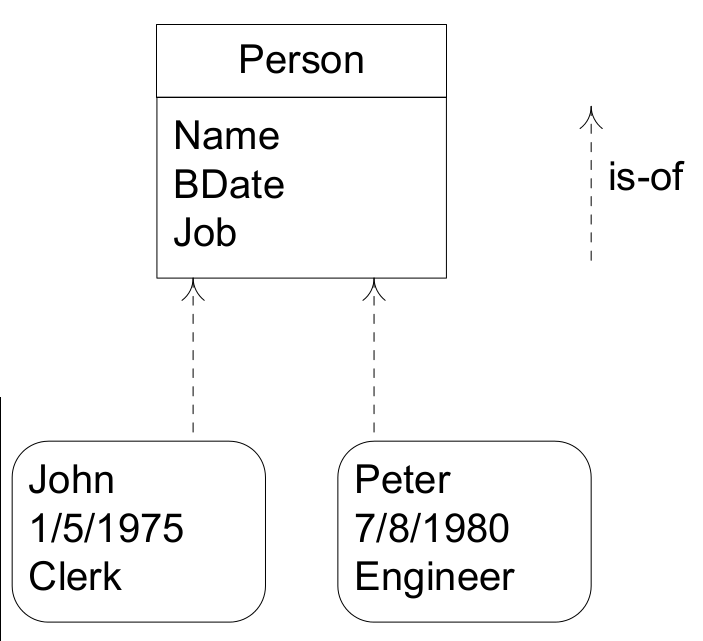
\includegraphics[width=.3\textwidth]{fig/entity.png}
    \caption{Une entité}
\end{figure}

\subsubsection{Attributs}
Les entités ont des attributs, qui ont une cardinalité minimale et maximale

\paragraph{Attributs multivalués}
Attributs dont la cardinalité maximale est supérieure à 1.
Exemple: \texttt{Person.degrees}

\paragraph{Attributs dérivés}
Attributs calculés à partir d'autres attributs, pas stockés dans la base de donnée.
Exemple: à partir du champ \texttt{Person.birth}, on peu déduire \texttt{Person.age}

\paragraph{Attributs composites}
Attributs formés par l'aggrégation de plusieurs autres attributs.
Exemple: \texttt{Person.Adress = \{Street, City, State, Zipcode, Country\}}

\paragraph{Clefs ou identificateurs}
Attributs ou ensemble d'attributs d'une entité dont les valeurs sont uniques
(déterminent une et une seule entité). On les met en évidence dans un schéma
entité-relation en les soulignant, en ajoutant un symbole \textit{clef} à côté,
ou en les mettant dans une section à part dans la boîte de l'entité.
\subparagraph{Clefs primaires}
Seule l'une des clefs peut être soulignée, et est l'identifiant d'un objet pour
cette entité.

\subsection{Relation}
\begin{figure}[h!]
    \center
    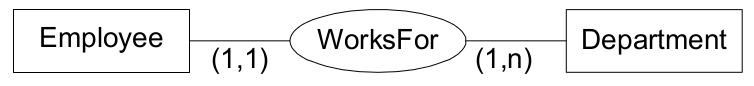
\includegraphics[width=.4\textwidth]{fig/relation.png}
    \caption{\label{fig:relation}Une relation One-to-many}
\end{figure}
\begin{figure}[h!]
    \center
    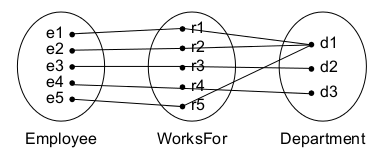
\includegraphics[width=.3\textwidth]{fig/relation-ensembliste.png}
    \caption{Vue ensembliste de la relation à la Figure \ref{fig:relation}}
\end{figure}
\begin{itemize}
  \item On doit spécifier la multiplicité minimale et maximale pour chaque pair de la relation
  \item La relation porte un nom (souvent lié au sens et à la sémantique de la relation)
  \item Chaque entité à un rôle dans la relation
  \item Une relation peut contenir des attributs
  \item L'arité ($x$-ary) d'une relation, ou son \textbf{degré}, indique le nombre d'entités participant à la relation
  \item \textbf{One-to-one}, \textbf{one-to-many} ou \textbf{many-to-many} pour les relations binaires
\end{itemize}

On peut noter qu'il n'y a pas de différence fondamentale entre un attribut et une relation,
juste une question de point de vue. On préfèrera une relation si on souhaite mettre en évidence
les liens entre plusieurs objets, et un attribut quand c'est une propriété comme un autre.

\subsubsection{Relation n-aire}
Une relation n-aire implique plus que 2 entités différentes.

\begin{figure}[h!]
    \center
    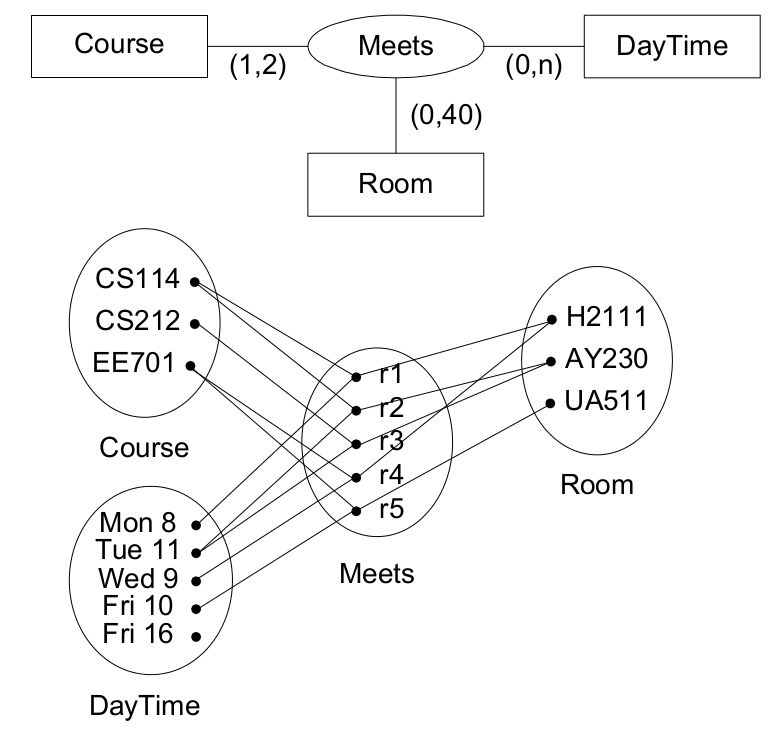
\includegraphics[width=.4\textwidth]{fig/relation-naire.png}
    \caption{Une relation ternaire et sa vue ensembliste}
\end{figure}

\subsubsection{Transformation des relation n-aires en binaires}
Les relations obtenues après transformation contiennent moins d'information
que la relation initiale. Par exemple, dans la Figure \ref{fig:relation-naire-projection},
on voit que la relation ternaire indique qu'un fournisseur délivre un produit pour un projet,
tandis que les relations binaires indiquent uniquement qu'un fournisseur délivre un produit,
qu'un projet utilise un produit, et qu'un projet utilise un fournisseur.

\paragraph{Projection}
On crée une relation pour chaque paire possible de la relation
\begin{figure}[h!]
    \center
    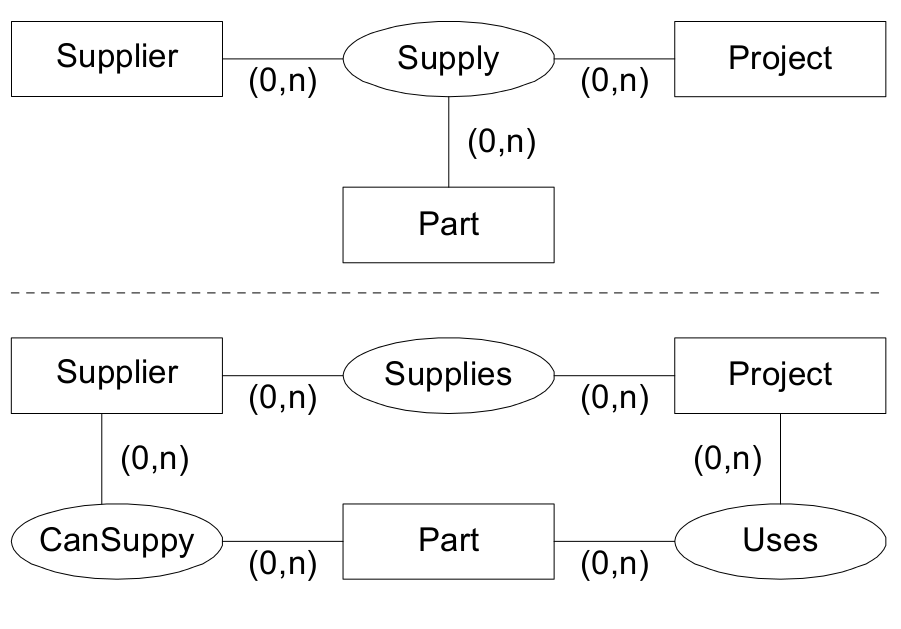
\includegraphics[width=.4\textwidth]{fig/relation-naire-projection.png}
    \caption{\label{fig:relation-naire-projection}Projection d'une relation ternaire}
\end{figure}

\paragraph{Insertion}
On transforme la relation en entité, et on la lie par des relations binaires à
toutes les entités de la relation initiale.
\begin{figure}[h!]
    \center
    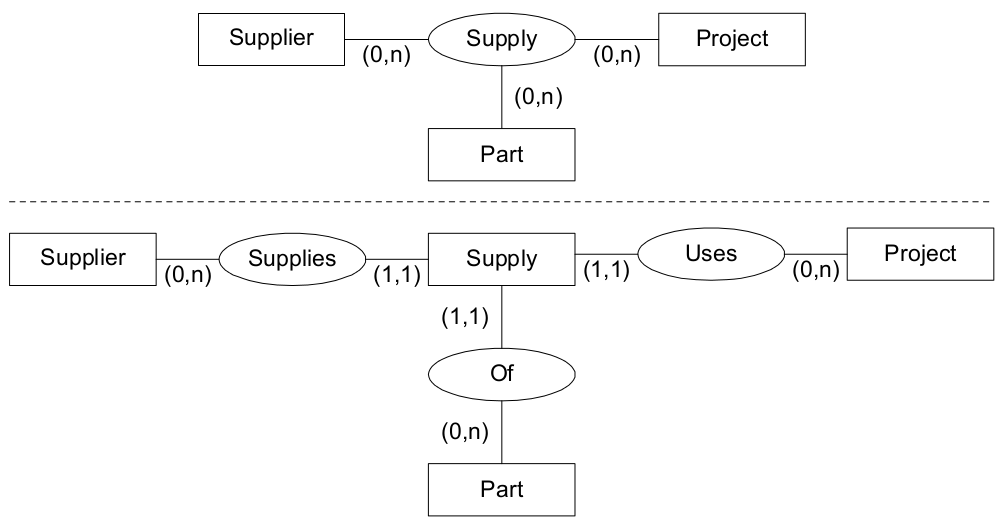
\includegraphics[width=.6\textwidth]{fig/relation-naire-insertion.png}
    \caption{Transformation par insertion}
\end{figure}

\subsection{Entités faibles}
Une entité faible n'a aucune clef ne dépendant que de ses propres attributs, et
a donc une \textbf{clef partielle} qui la distingue des autres entités ayant la
même clef étrangère.

\end{document}